\chapter{Examples}
\label{cha:examples}


This chapter contains a few another examples from the literature
dealing with chemical reactors. The examples were choosen to
illustrate the ability of the~\fun{dynopt} package to treat the
problems of varying levels of difficulty. The example files can be
found in the directory~\subor{examples/problemX}, where X means the
number of the problem presented in this chapter.

\section{Problem 4}
\label{sec:prob4}

Consider a tubular reactor with  parallel
reactions $A \rightarrow B$, $A \rightarrow C$ taking place
\citep{raj01,dad95,log89}:
\begin{equation}
\max_{\ve{u}(t)} \mf{J} = x_{2}(t_{f}) \label{eq:tubular}
\end{equation}
such that
\begin{align*}
\dot{x}_1 &=-(u+0.5u^2)x_{1} &x_1(0) &= 1 \\
\dot{x}_2 &=ux_1 &x_2(0) &= 0 \\
u &\in [0,5] & t_f &=1
\end{align*}
where 
\begin{description}
\item $x_{1}(t)$ -- dimensionless concentration of A,
\item $x_{2}(t)$ -- dimensionless concentration of B,
\item $u(t)$ -- control variable.
\end{description}

This problem was treated by~\cite{dad95,log89,raj01} and the value of
performance index of value of 0.57353 was reported as global optimum
by \cite{dad95}. Moreover the value of 0.57284 was reported by
\cite{raj01}. By using 6 collocation points for state variables, 2  
collocation points for control variables on the same number of
intervals as in the literature to this problem, we obtained a slightly
closer value of performance index of 0.57310 to the reported global
maximum. The optimal control and state profiles are given in
Figs. \ref{fig:prob4_u} and \ref{fig:prob4_x}.

\begin{figure}[htb]
\begin{minipage}[t]{0.5\linewidth}
\centering
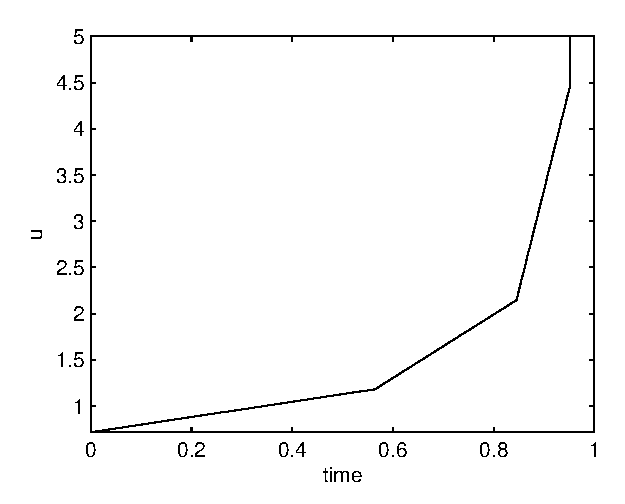
\includegraphics[width=0.9\textwidth]{examples/problem4/graphs/u_624a.eps}
\caption[Problem 4: Control profile]{Control profile for problem 4}
\label{fig:prob4_u}  
\end{minipage}
\begin{minipage}[t]{0.5\linewidth}
\centering
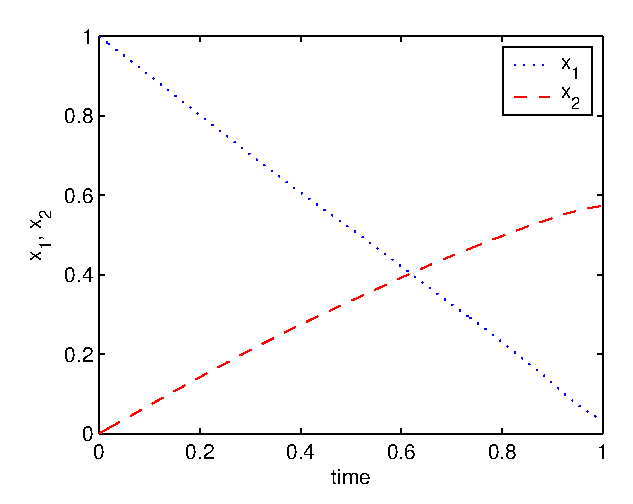
\includegraphics[width=0.9\textwidth]{examples/problem4/graphs/x12_624a.eps}
\caption[Problem 4: State profiles]{State profiles for problem 4}
\label{fig:prob4_x} 
\end{minipage}
\end{figure}
 
\section{Problem 5}
\label{sec:prob5}

Consider a batch reactor~\citep{raj01,dad95} where a series of
reactions $A \rightarrow B\rightarrow C$ is involved. This example is
similar to that in section \ref{sec:brpdae}. The difference is just in
the reactor model description. Here the process is described as an ODE
system.  
\begin{equation}
\max_{\ve{u}(t)} \mf{J} = x_{2}(t_{f}) \label{eq:batch}
\end{equation}
such that
\begin{align*}
\dot{x}_1&=-k_{1}x_{1}^{2} &x_1(0) &= 1 \\
\dot{x}_2&=k_{1}x_{1}^{2}-k_{2}x_{2} &x_2(0) &= 0 \\
k_1 &=4000e^{(-\frac{2500}{T})} &k_2 &=620000e^{(-\frac{5000}{T})} \\
T &\in [298,398] & t_f &=1
\end{align*}
where
\begin{description}
\item $x_{1}(t)$ -- concentration of A,
\item $x_{2}(t)$ -- concentration of B,
\item $T$ -- temperature (control variable).
\end{description}

The objective of problem~\eqref{eq:batch} is to obtain the optimal
temperature profile that maximises the yield of the intermediate
product B at the end of a specified time of operation in a batch
reactor where the reaction  $A \rightarrow B \rightarrow C$ take
place. The problem was solved using a relaxed reduced space SQP
strategy by~\cite{log89} and the value of 0.610775 was reported as
global maximum.~\citeauthor{raj01} reached the value of 0.61045. We
obtained optimal value of 0.610756, by using 5 collocation points for
state variables and keeping control variable profile as piecewise
linear on 4 time intervals. This is quite closer to the global
one. The optimal control and state profiles are given in
Figs.~\ref{fig:prob5_u} and \ref{fig:prob5_x}. 
  
\begin{figure}[htb]
\begin{minipage}[t]{0.5\linewidth}
\centering
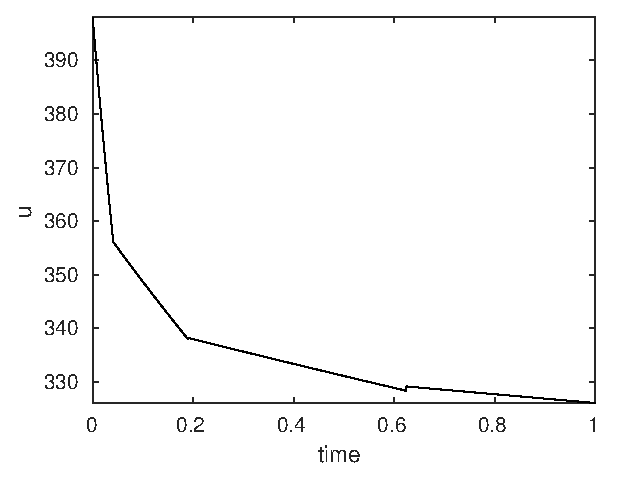
\includegraphics[width=0.9\textwidth]{examples/problem5/graphs/u_524a.eps}
\caption[Problem 5: Control profile]{Control profile for problem 5}
\label{fig:prob5_u}  
\end{minipage}
\begin{minipage}[t]{0.5\linewidth}
\centering
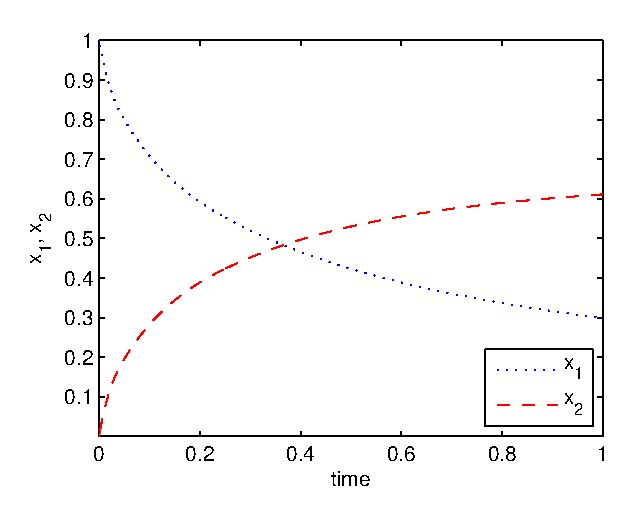
\includegraphics[width=0.9\textwidth]{examples/problem5/graphs/x12_524a.eps}
\caption[Problem 4: State profiles]{State profiles for problem 5}
\label{fig:prob5_x} 
\end{minipage}
\end{figure}

\section{Problem 6}
\label{sec:prob6}

Consider a catalytic plug flow reactor~\citep{raj01,dad95} involving
the following reactions:\\ 
$A \leftrightarrow B\rightarrow C$
\begin{equation}
\max_{\ve{u}(t)} \mf{J} = 1-x_{1}(t_{f})-x_{2}(t_{f})
\label{eq:plugflow} 
\end{equation}
such that
\begin{align*}
\dot{x}_1&=u(10x_2-x_1) &x_1(0) &= 1 \\
\dot{x}_2&=-u(10x_2-x_1)-(1-u)x_2  &x_2(0) &= 0 \\
u &\in [0,1] & t_f &=12
\end{align*}
where
\begin{description}
\item $x_1(t)$ -- mole fraction of A,
\item $x_2(t)$ -- mole fraction of B,
\item $u(t)$ -- fraction of type 1 catalyst.
\end{description}

Optimisation of this problem has also been analysed. This problem was
solved by~\cite{log89,raj01} and the optima 0.476946, 0.47615 were
reported. Value of the performance index obtained for this problem
using~\fun{dynopt} was 0.477456. In this case 5 collocation points for
state variables and 2 collocation points for control variables were
choosen. The number of time-intervals have been set to 12. The optimal
control and state profiles are given in Figs.~\ref{fig:prob6_u} and
\ref{fig:prob6_x}.  

\begin{figure}[htb]
\begin{minipage}[t]{0.5\linewidth}
\centering
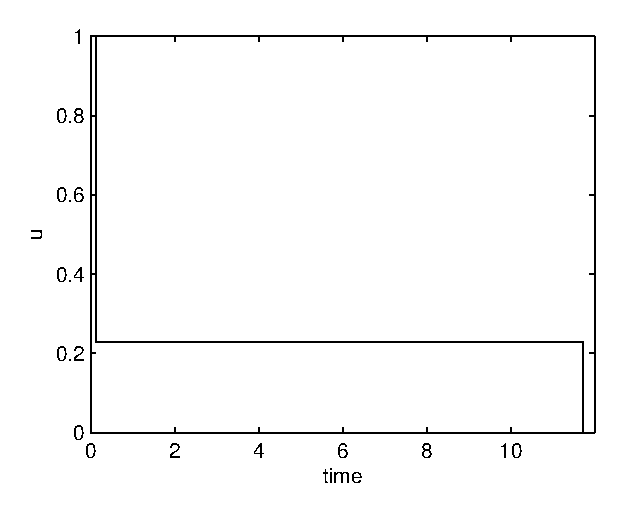
\includegraphics[width=0.9\textwidth]{examples/problem6/graphs/u_5212a.eps}
\caption[Problem 6: Control profile]{Control profile for problem 6}
\label{fig:prob6_u} 
\end{minipage}
\begin{minipage}[t]{0.5\linewidth}
\centering
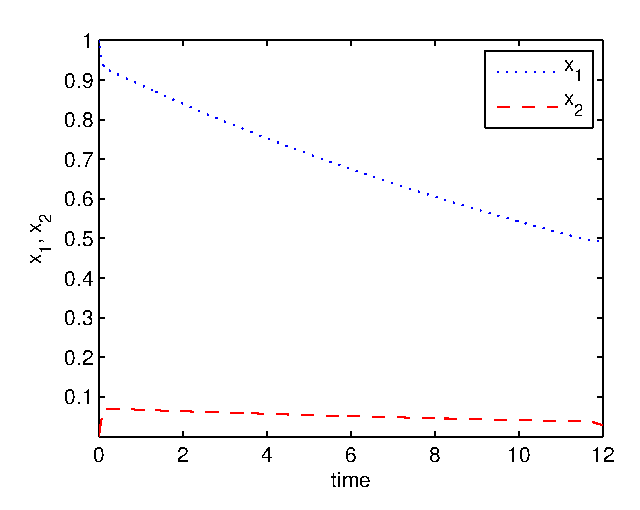
\includegraphics[width=0.9\textwidth]{examples/problem6/graphs/x12_5212a.eps}
\caption[Problem 6: State profiles]{State profiles for problem 6}
\label{fig:prob6_x}  
\end{minipage}
\end{figure}

\section{Problem 7}
\label{sec:prob7}

Consider the following problem~\citep{luu90_52,bal01,fik02} 

\begin{gather}
\max_{\ve{u}(t)} \mf{J} =
\int_{0}^{0.2}\big(5.8(qx_{1}-u_{4})-3.7u_{1}-4.1u_{2}\nonumber\\ % x_{8}\label{eq:e5} 
\mbox{}+q(23x_{4}+11x_{5}+28x_{6}+35x_{7})-5.0u_{3}^{2}\nonumber\\
\mbox{}-0.099\big)\dt \label{eq:cstr}
\end{gather}
such that
\begin{gather*}
\dot{x}_1  =  u_{4}-qx_{1}-17.6x_{1}x_{2}-23x_{1}x_{6}u_{3}\\
\dot{x}_2  =  u_{1}-qx_{2}-17.6x_{1}x_{2}-146x_{2}x_{3}\\
\dot{x}_3  =  u_{2}-qx_{3}-73x_{2}x_{3}\\
\dot{x}_4  =  -qx_{4}+35.2x_{1}x_{2}-51.3x_{4}x_{5}\\
\dot{x}_5  =  -qx_{5}+219x_{2}x_{3}-51.3x_{4}x_{5}\\
\dot{x}_6  =  -qx_{6}+102.6x_{4}x_{5}-23x_{1}x_{6}u_{3}\\
\dot{x}_7  =  -qx_{7}+46x_{1}x_{6}u_{3}\\
% \dot{x}_8  =  5.8(qx_{1}-u_{4})-3.7u_{1}-4.1u_{2}+{}\\
% {}+q(23x_{4}+11x_{5}+28x_{6}+35x_{7})-5.0u_{3}^{2}-0.099\\
\ve{x}(0) = [0.1883~0.2507~0.0467~0.0899~0.1804~0.1394~0.1046]^{\textrm{T}}\\
q = u_{1}+u_{2}+u_{4}\\
0 \leq u_{1} \leq 20\\
0 \leq u_{2} \leq 6\\
0 \leq u_{3} \leq 4\\
0 \leq u_{4} \leq 20\\
t_{f}=0.2
\end{gather*}
where 
\begin{description}
\item $x_{1}(t) - x_{7}(t)$ -- states,
\item $u_{1}(t) - u_{4}(t)$ -- controls.
\end{description}
Analogous to the section \ref{sec:statepathconprob}, the cost function
can be rewritten to the Mayer form by introducing a new state defined
by the integral function with its initial value equal to zero.

This problem was solved by~\cite{fik02,jac69}. Reported optimal value
of 21.757 was obtained using CVP method implemented in DYNO. For this
problem, 4 collocation points for state variables, 2 collocation
points for control variables for 10 intervals were defined and an
optimum was found at value of 21.8003. The optimal control profiles
are given in Figs. \ref{fig:prob7_u1}, \ref{fig:prob7_u2},
\ref{fig:prob7_u3}, \ref{fig:prob7_u4} and optimal state profiles are
represented in Fig.~\ref{fig:prob7_x}.  

\begin{figure}[htb]
\begin{minipage}[t]{0.5\linewidth}
\centering
\includegraphics[width=0.9\textwidth]{examples/problem7/graphs/u1_4210.eps}
\caption[Problem 7: Control profile for $u_{1}$]{Control $u_{1}$ for
  problem 7} \label{fig:prob7_u1} 
\end{minipage}
\begin{minipage}[t]{0.5\linewidth}
\centering
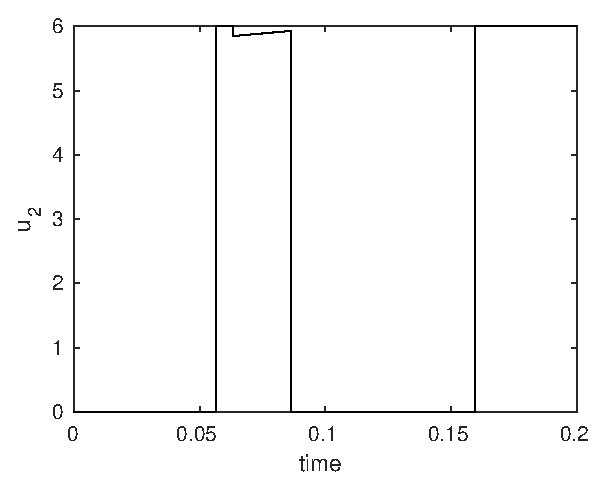
\includegraphics[width=0.9\textwidth]{examples/problem7/graphs/u2_4210.eps}
\caption[Problem 7: Control profile for $u_{2}$]{Control $u_{2}$ for
  problem 7} \label{fig:prob7_u2} 
\end{minipage}
\begin{minipage}[t]{0.5\linewidth}
\centering
\includegraphics[width=0.9\textwidth]{examples/problem7/graphs/u3_4210.eps}
\caption[Problem 7: Control profile for $u_{3}$]{Control $u_{3}$ for
  problem 7} \label{fig:prob7_u3} 
\end{minipage}
\begin{minipage}[t]{0.5\linewidth}
\centering
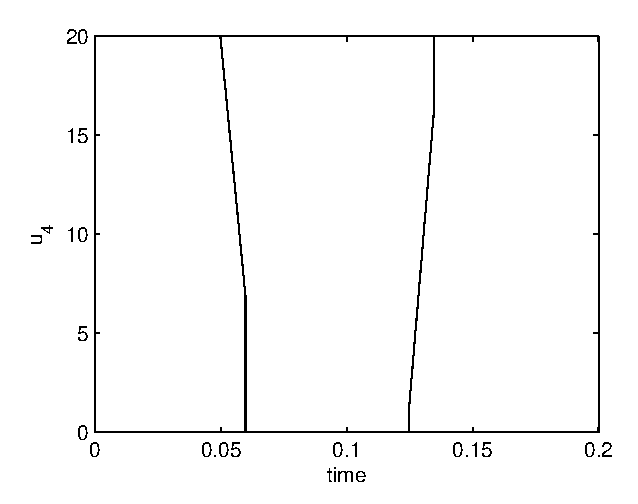
\includegraphics[width=0.9\textwidth]{examples/problem7/graphs/u4_4210.eps}
\caption[Problem 7: Control profile for $u_{4}$]{Control $u_{4}$ for
  problem 7} \label{fig:prob7_u4}
\end{minipage}
\begin{minipage}[t]{0.5\linewidth}
\centering
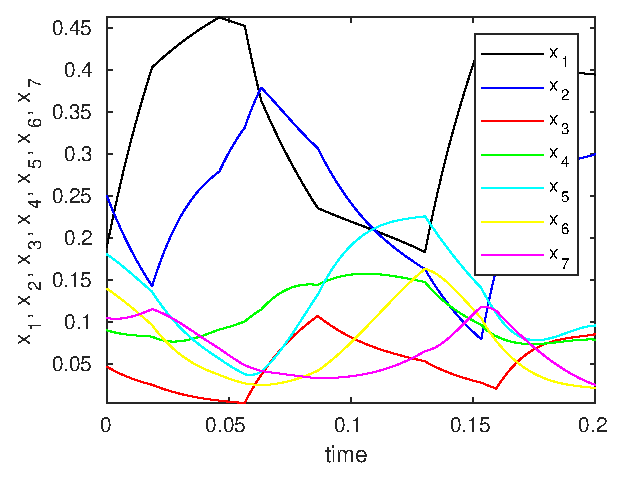
\includegraphics[width=0.9\textwidth]{examples/problem7/graphs/x17_4210.eps}
\caption[Problem 7: State profiles]{State profiles for problem 7}
\label{fig:prob7_x} 
\end{minipage}
\end{figure}



%%% Local Variables: 
%%% mode: latex
%%% TeX-master: "dynopt_guide"
%%% End: 
